
The deployment of deep learning models trained on synthetic data to real-world environments represents one of the most significant challenges in modern computer vision and robotics. This chapter provides a comprehensive treatment of the domain gap problem, examining both theoretical foundations and practical methodologies for bridging the divide between simulated and physical domains. The techniques presented herein form the theoretical backbone for reinforcement learning-based optimization of synthetic data generation parameters, enabling autonomous systems to achieve robust performance on real-world perception tasks without requiring extensive manually-labeled datasets.

\begin{figure}[htbp]
\centering
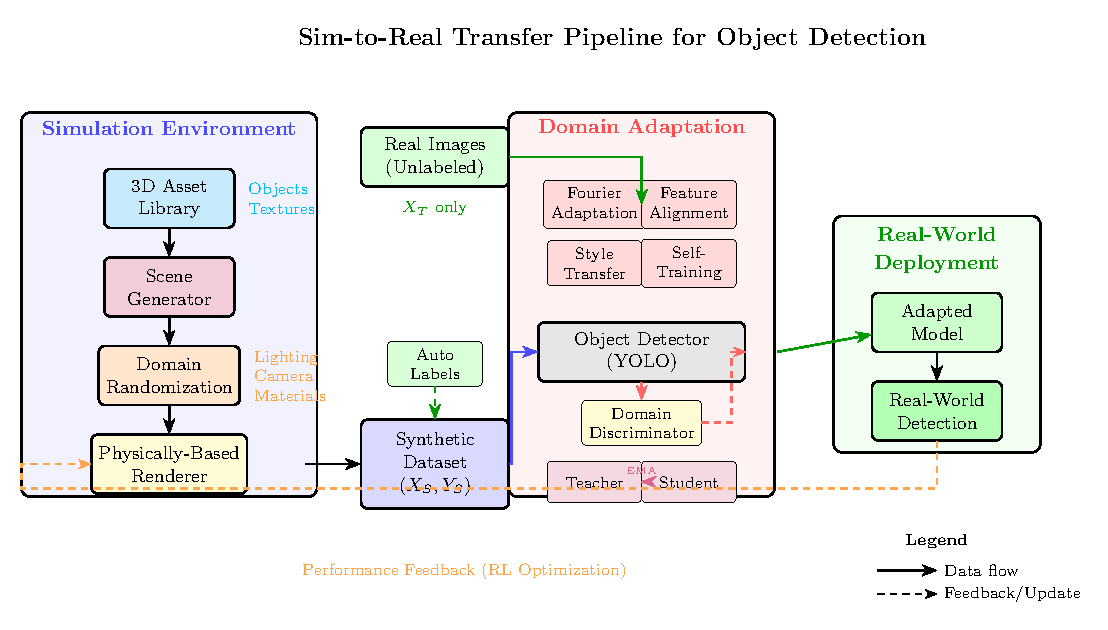
\includegraphics[width=\textwidth]{figures/ch06_fig2_simtoreal_pipeline.pdf}
\caption{Overview of the sim-to-real transfer pipeline for object detection. Synthetic data generated in simulation environments undergoes domain adaptation techniques before training object detectors. The adapted models are then deployed in real-world settings, with performance feedback potentially informing refinement of the synthetic data generation process through reinforcement learning optimization.}
\label{fig:simtoreal_pipeline}
\end{figure}

\section{The Domain Gap Problem}
\label{sec:domain_gap_problem}

The fundamental challenge of transferring knowledge from synthetic to real domains stems from distributional differences that arise from the inherent limitations of simulation environments. Understanding the mathematical formulation of this gap, its sources, and methods for quantification provides essential groundwork for developing effective mitigation strategies.

\begin{figure}[htbp]
\centering
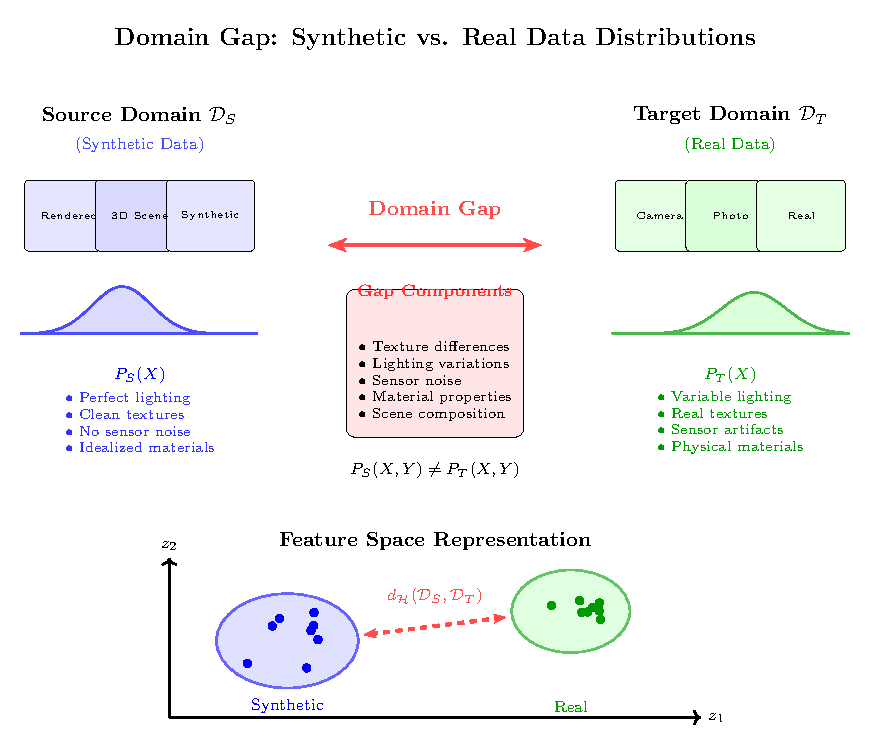
\includegraphics[width=\textwidth]{figures/ch06_fig1_domain_gap.pdf}
\caption{Visualization of the domain gap between synthetic and real data distributions. The source domain $\mathcal{D}_S$ (synthetic) and target domain $\mathcal{D}_T$ (real) exhibit different marginal distributions $P_S(X)$ and $P_T(X)$. Key gap components include texture differences, lighting variations, sensor noise characteristics, and scene composition. The bottom panel shows how this gap manifests in learned feature space, where synthetic and real samples form separated clusters with measurable distance $d_{\mathcal{H}}(\mathcal{D}_S, \mathcal{D}_T)$.}
\label{fig:domain_gap_viz}
\end{figure}

\subsection{Formal Definition of Domain Shift}

Consider a source domain $\mathcal{D}_S$ representing synthetic data and a target domain $\mathcal{D}_T$ representing real-world observations. Each domain is characterized by a joint probability distribution over input features $\mathcal{X}$ and labels $\mathcal{Y}$. The source domain distribution is denoted $P_S(X, Y)$ while the target domain distribution is $P_T(X, Y)$. Domain shift occurs when these distributions differ, mathematically expressed as $P_S(X, Y) \neq P_T(X, Y)$.

This distributional discrepancy can be decomposed into several components. Covariate shift arises when the marginal distributions differ, $P_S(X) \neq P_T(X)$, while the conditional distribution remains constant, $P_S(Y|X) = P_T(Y|X)$. Label shift occurs in the reverse scenario where $P_S(Y) \neq P_T(Y)$ but $P_S(X|Y) = P_T(X|Y)$. The most challenging case involves concept drift where both marginal and conditional distributions differ simultaneously.

\begin{definition}[Domain Gap]
\label{def:domain_gap}
Let $\mathcal{H}$ be a hypothesis class and let $h \in \mathcal{H}$ be a predictor. The domain gap $d_{\mathcal{H}}(\mathcal{D}_S, \mathcal{D}_T)$ is defined as the supremum over the hypothesis class of the difference in expected losses:
\begin{equation}
d_{\mathcal{H}}(\mathcal{D}_S, \mathcal{D}_T) = \sup_{h \in \mathcal{H}} \left| \mathbb{E}_{(x,y) \sim P_S}[\ell(h(x), y)] - \mathbb{E}_{(x,y) \sim P_T}[\ell(h(x), y)] \right|
\end{equation}
where $\ell(\cdot, \cdot)$ denotes the task-specific loss function.
\end{definition}

The implications of domain shift for object detection are particularly severe. A detector trained exclusively on synthetic renderings may exhibit dramatically degraded performance when deployed on real camera imagery due to systematic differences in texture statistics, illumination characteristics, sensor noise profiles, and contextual scene composition.

\subsection{Sources of Sim-to-Real Gap}

The discrepancy between synthetic and real visual domains originates from multiple interacting factors that span the rendering pipeline, environmental modeling, and sensor simulation. Understanding these sources enables targeted intervention strategies.

Texture fidelity represents a primary contributor to domain gap. Synthetic rendering engines, despite advances in physically-based rendering, produce texture patterns that differ systematically from real-world surface appearances. Material reflectance properties including bidirectional reflectance distribution functions are approximated rather than measured, leading to subtle but perceptually significant deviations. Research by Geirhos et al. demonstrated that convolutional neural networks exhibit strong texture bias, relying on local texture patterns for classification rather than global shape information. This bias amplifies the impact of texture discrepancies between domains, as networks trained on synthetic textures may fail to recognize objects with different but semantically equivalent surface appearances.

Illumination modeling introduces systematic biases through simplified light transport simulation. Real-world scenes exhibit complex interreflection, subsurface scattering, and atmospheric effects that are computationally expensive to simulate accurately. Synthetic environments typically employ a limited number of point or area light sources with idealized emission profiles, whereas natural environments feature continuous illumination from the sky dome, diffuse inter-object reflections, and spatially varying ambient conditions. The resulting differences in shadow characteristics, highlight patterns, and overall luminance distributions contribute significantly to domain gap.

Sensor noise characteristics differ fundamentally between simulated and physical imaging systems. Real cameras exhibit spatial noise patterns arising from pixel-level variations in sensitivity, temporal noise from electronic readout circuits, and photon shot noise following Poisson statistics. Color reproduction depends on spectral response curves of physical sensors that deviate from idealized RGB filters assumed in rendering. Lens aberrations including chromatic dispersion, vignetting, and geometric distortion are present in physical optics but typically absent from synthetic rendering.

Contextual scene composition presents challenges in ensuring that synthetic environments capture the statistical regularities of real-world object arrangements. Objects in physical environments follow implicit placement rules governed by physics, human design intent, and functional relationships. Vehicles appear on roads rather than arbitrary locations; products occupy shelves in retail environments; pedestrians traverse sidewalks and crosswalks. Violating these contextual priors in synthetic data generation produces training examples that are implausible under the real-world distribution, potentially teaching detectors spurious correlations.

\subsection{Measuring Domain Gap}

Quantitative assessment of domain discrepancy enables systematic comparison of synthetic data generation strategies and provides feedback signals for optimization-based approaches. Several metrics have been proposed for measuring distributional divergence between image domains.

The Fr\'{e}chet Inception Distance provides a widely-adopted measure of distributional similarity between image collections. Given feature representations extracted from a pretrained Inception network, FID models both synthetic and real feature distributions as multivariate Gaussians and computes the Fr\'{e}chet distance between them:
\begin{equation}
\text{FID} = \|\mu_S - \mu_T\|_2^2 + \text{Tr}\left(\Sigma_S + \Sigma_T - 2(\Sigma_S \Sigma_T)^{1/2}\right)
\end{equation}
where $\mu_S, \Sigma_S$ and $\mu_T, \Sigma_T$ denote the mean vectors and covariance matrices of source and target feature distributions respectively. Lower FID values indicate greater distributional similarity. While FID correlates with human perceptual judgments of image quality, it exhibits statistical bias when computed from limited sample sizes, requiring collections of fifty thousand or more images for reliable estimation.

The Kernel Inception Distance addresses the sample efficiency limitations of FID by employing Maximum Mean Discrepancy in the feature space. KID provides an unbiased estimator that yields reliable measurements from smaller image collections:
\begin{equation}
\text{KID} = \mathbb{E}[k(\phi(x_S), \phi(x'_S))] + \mathbb{E}[k(\phi(x_T), \phi(x'_T))] - 2\mathbb{E}[k(\phi(x_S), \phi(x_T))]
\end{equation}
where $\phi(\cdot)$ denotes the Inception feature extractor and $k(\cdot, \cdot)$ is a polynomial or Gaussian kernel function. The unbiased nature of KID makes it particularly suitable for iterative optimization scenarios where computational constraints limit the number of synthetic images generated per evaluation.

Maximum Mean Discrepancy provides a general framework for comparing probability distributions in reproducing kernel Hilbert spaces. Given kernel function $k$, the squared MMD between distributions $P$ and $Q$ is:
\begin{equation}
\text{MMD}^2(P, Q) = \left\| \mathbb{E}_{x \sim P}[\phi(x)] - \mathbb{E}_{y \sim Q}[\phi(y)] \right\|_{\mathcal{H}}^2
\end{equation}
where $\phi$ maps samples to the RKHS induced by kernel $k$. MMD can be computed efficiently using kernel evaluations without explicit feature mapping, enabling application to high-dimensional image distributions.

The Style Embedding Distribution Discrepancy metric specifically targets the synthetic-real gap by modeling domain differences as style variations. SEDD extracts style representations using Gram matrices of intermediate convolutional features and measures discrepancy through a learned embedding space optimized for intra-class compactness and inter-class separation. This approach captures texture and appearance statistics that are particularly relevant for sim-to-real transfer.

\subsection{Feature Space Analysis Methods}

Beyond scalar metrics, visualization and analysis of learned feature representations provide insight into the geometric structure of domain gap in representation space.

t-distributed Stochastic Neighbor Embedding enables projection of high-dimensional feature vectors to two-dimensional visualizations that preserve local neighborhood structure. By extracting backbone features from both synthetic and real images and projecting them jointly via t-SNE, practitioners can visually assess the degree of domain alignment. Well-aligned domains exhibit overlapping clusters in the projected space, while substantial domain gap manifests as separated clusters corresponding to synthetic and real origins. Class-conditional visualization reveals which object categories exhibit the largest domain discrepancy, enabling targeted improvement of synthetic data generation for problematic classes.

Layer-wise analysis of feature distributions across network depth provides diagnostic information about where domain-specific information persists in learned representations. Shallow layers typically exhibit greater separation between synthetic and real features due to their sensitivity to low-level image statistics including edges, textures, and color distributions. Deeper layers ideally produce more domain-invariant representations that capture semantic content rather than domain-specific appearance. Persistent domain separation in deep layers indicates insufficient domain adaptation, suggesting the need for explicit alignment mechanisms or improved synthetic data diversity.

Principal Component Analysis of feature spaces reveals the principal directions of variation and enables quantification of how much variance is explained by domain identity versus semantic content. If the first principal components separate domains rather than semantic categories, the learned representations are dominated by domain-specific rather than task-relevant information.

\section{Domain Randomization Theory}
\label{sec:dr_theory}

Domain randomization provides a conceptually elegant approach to sim-to-real transfer by deliberately introducing variation during synthetic data generation such that the real world appears as merely another sample from the training distribution. This section establishes the theoretical foundations of domain randomization and derives conditions under which it enables successful transfer.

\subsection{Theoretical Foundations}

The seminal work of Tobin et al. established the empirical effectiveness of domain randomization for robotic manipulation, demonstrating successful transfer of neural network policies trained entirely on synthetic RGB images to physical robot systems. The core insight underlying domain randomization is that by exposing the learning system to sufficient variability in non-essential visual parameters, it is forced to learn representations that are invariant to these nuisance factors and therefore more likely to generalize to novel visual conditions including those encountered in real deployments.

Formal theoretical analysis of domain randomization was provided by subsequent work establishing mathematical foundations for understanding when and why randomization enables generalization. Consider a simulator $\mathcal{S}$ parameterized by environment parameters $\xi \in \Xi$ drawn from distribution $\rho(\xi)$. The goal is to learn a policy or predictor $\pi$ that performs well under the real-world parameter instantiation $\xi^*$.

\begin{theorem}[Domain Randomization Transfer Bound]
\label{thm:dr_transfer}
Let $\pi$ be a predictor trained on synthetic data generated with environment parameters drawn from $\rho(\xi)$. Under the assumption that $\xi^* \in \text{supp}(\rho)$ and that the learned representation $\phi$ satisfies a Lipschitz condition with constant $L_\phi$, the expected loss on the target domain is bounded by:
\begin{equation}
\mathbb{E}_{(x,y) \sim P_T}[\ell(\pi(x), y)] \leq \mathbb{E}_{\xi \sim \rho}\mathbb{E}_{(x,y) \sim P_\xi}[\ell(\pi(x), y)] + L_\phi \cdot \mathbb{E}_{\xi \sim \rho}[d(\xi, \xi^*)]
\end{equation}
where $d(\cdot, \cdot)$ measures distance in parameter space and $P_\xi$ denotes the data distribution under parameter $\xi$.
\end{theorem}

This bound reveals the fundamental tradeoff in domain randomization. Broader parameter distributions $\rho$ increase the likelihood that real-world conditions fall within support while potentially increasing the average distance term. Conversely, narrow distributions centered near presumed real-world parameters minimize distance but risk excluding actual deployment conditions from the training distribution.

\begin{figure}[htbp]
\centering
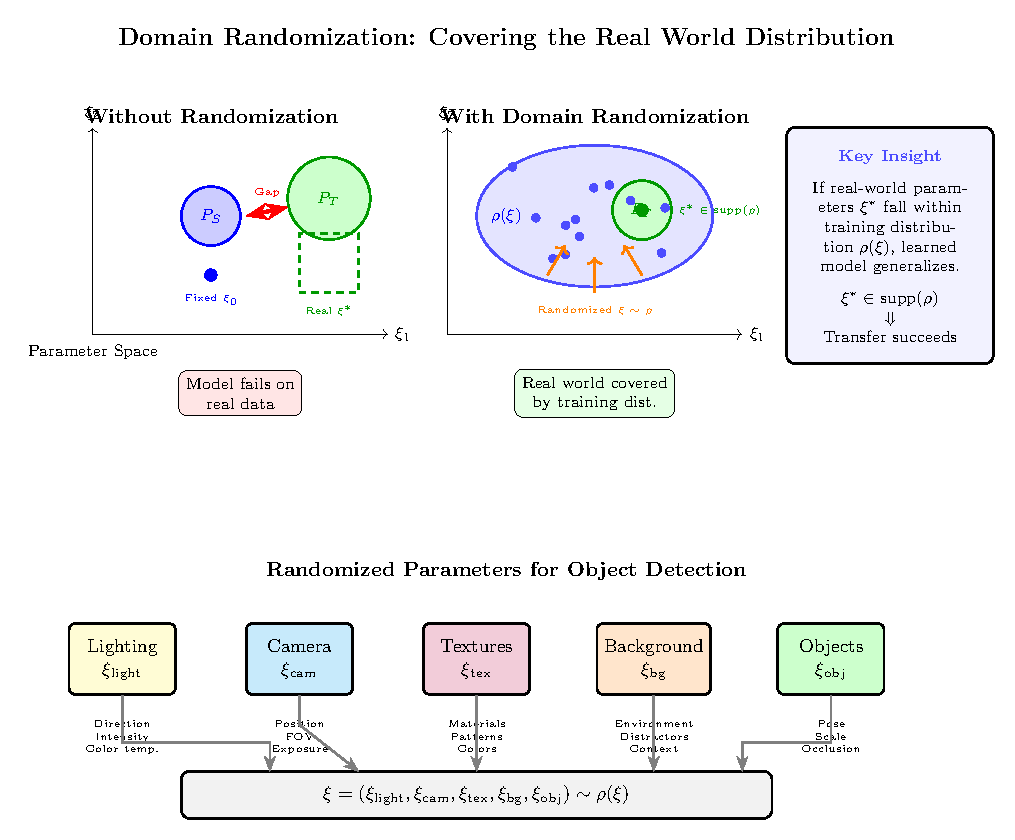
\includegraphics[width=\textwidth]{figures/ch06_fig3_domain_randomization.pdf}
\caption{The domain randomization principle for sim-to-real transfer. Without randomization (left), the narrow synthetic distribution $P_S$ fails to cover the real-world distribution $P_T$, resulting in poor transfer. With domain randomization (center), the training distribution $\rho(\xi)$ is broadened across environment parameters to encompass real-world conditions, ensuring $\xi^* \in \text{supp}(\rho)$. The bottom panel illustrates the key randomization parameters for object detection including lighting, camera pose, textures, backgrounds, and object configurations.}
\label{fig:domain_randomization}
\end{figure}

The ICLR 2022 framework for understanding domain randomization established that history-dependent policies utilizing memory or recurrence are essential for achieving tight transfer bounds. Memoryless policies cannot distinguish between environment parameters and must hedge against all possible parameter values, leading to conservative suboptimal behavior. In contrast, recurrent architectures can infer environment parameters from sequential observations and adapt their behavior accordingly, achieving near-optimal performance across the randomization distribution.

\subsection{Why Randomization Enables Generalization}

The generalization mechanism of domain randomization operates through several complementary effects on learned representations.

Invariance learning arises when parameters randomized during training are held constant within individual training episodes or images but vary across the dataset. The network cannot rely on randomized parameters for prediction since their values are unpredictable, forcing it to learn features that remain discriminative regardless of these nuisance variables. This mechanism mirrors the classical computer vision principle of designing features invariant to illumination, viewpoint, and other imaging conditions.

Distribution coverage ensures that real-world conditions fall within the training distribution when randomization ranges are sufficiently broad. From the perspective of empirical risk minimization, training on a distribution that covers the test distribution provides guarantees on generalization through standard learning theory arguments. The real world becomes just another sample from an already-observed distribution rather than an out-of-distribution extrapolation.

Regularization effects emerge from the increased training distribution entropy induced by randomization. Similar to data augmentation, domain randomization can be viewed as implicit regularization that prevents overfitting to specific visual conditions present in a narrow synthetic distribution. This regularization effect improves generalization even to conditions outside the explicit randomization ranges.

Meta-learning dynamics arise when randomization creates a distribution over distinct training environments. Memory-augmented architectures can learn to identify environment parameters from observations and adapt their processing accordingly, implementing a form of meta-learning where the network learns how to learn about new environments. This enables rapid adaptation to deployment conditions that may differ from any specific training environment.

\subsection{Optimal Randomization Ranges}

Determining appropriate ranges for randomized parameters involves balancing competing considerations. Ranges that are too narrow risk excluding real-world conditions, while excessively broad ranges increase training difficulty and may lead to overly conservative learned representations.

Empirical guidelines derived from successful applications suggest parameter-specific recommendations. Camera position should be randomized within task-relevant viewing volumes, typically spanning elevation angles from five to thirty degrees and full azimuthal coverage for objects that may be approached from any direction. Lighting parameters benefit from randomization across one to twelve light sources with log-uniform intensity distributions spanning an order of magnitude around nominal values. Background textures should be sampled from diverse image databases containing thousands of distinct patterns to ensure coverage of texture statistics encountered in deployment.

The principle of physicality constrains randomization to plausible parameter combinations. While broad marginal distributions for individual parameters may be desirable, joint distributions should respect physical constraints. Light source positions and shadow directions must be consistent. Object textures and reflectance properties should correspond to materials plausibly associated with the object category. Gravity-consistent object arrangements avoid floating or intersecting configurations that could never occur in physical environments.

Curriculum strategies for range selection begin with conservative ranges that enable initial learning and progressively expand as training progresses. This approach, formalized in automatic domain randomization methods, avoids the difficulty of learning from maximally diverse distributions while eventually achieving broad coverage.

\subsection{The Exploration-Robustness Tradeoff}

Domain randomization fundamentally trades task performance for robustness across environmental conditions. This tradeoff manifests in several ways that practitioners must navigate.

Conservative policies emerge when training under broad randomization because the learned system must hedge against all possible parameter values. A policy optimized for average performance across a wide parameter distribution will typically underperform compared to a policy specialized for specific known conditions. This suboptimality is the price paid for robustness.

Training difficulty increases with randomization breadth as the learning problem becomes more challenging. The network must simultaneously master the task and achieve invariance to randomized parameters. Combined randomization of many parameters creates a high-dimensional space of training conditions that may require substantially more training data and computational resources to cover adequately.

Diminishing returns characterize the relationship between randomization breadth and sim-to-real transfer performance. Initial randomization provides substantial benefits by breaking dependence on simulation-specific artifacts. However, beyond a threshold, additional randomization primarily increases training difficulty without proportionate gains in transfer performance, particularly when real-world conditions already fall within established ranges.

\begin{theorem}[Exploration-Robustness Tradeoff]
\label{thm:exploration_robustness}
Let $\rho_\sigma$ denote a randomization distribution with scale parameter $\sigma$ and let $R(\pi, \xi)$ denote the expected return of policy $\pi$ under environment parameter $\xi$. The robust expected return and the optimal specialized return satisfy:
\begin{equation}
\mathbb{E}_{\xi \sim \rho_\sigma}[R(\pi^*_\sigma, \xi)] \leq \max_\xi R(\pi^*_\xi, \xi) - \Omega(\sigma)
\end{equation}
where $\pi^*_\sigma$ is optimal under randomization and $\pi^*_\xi$ is optimal for specific $\xi$. The gap grows with randomization scale $\sigma$.
\end{theorem}

This theorem formalizes the intuition that robustness comes at the cost of peak performance. Practitioners must determine acceptable tradeoffs based on the relative importance of average-case versus worst-case performance in their application domain.

\section{Structured Domain Randomization}
\label{sec:structured_dr}

While uniform domain randomization provides a simple baseline, structured approaches that incorporate prior knowledge about realistic scene configurations achieve superior transfer performance with improved sample efficiency.

\subsection{NVIDIA's SDR Approach}

Structured Domain Randomization, introduced by NVIDIA researchers, represents a principled framework for incorporating contextual constraints into synthetic data generation. Rather than placing objects according to uniform distributions over spatial coordinates, SDR samples object configurations from distributions that reflect the statistical regularities of real-world scenes.

The key insight motivating SDR is that random placement of objects in arbitrary locations produces training examples that violate the implicit assumptions of real-world imagery. Vehicles appearing in the sky, pedestrians embedded in walls, and products floating above shelves represent configurations that never occur in deployment yet consume training capacity when included in uniformly randomized datasets. By restricting randomization to contextually appropriate variations, SDR focuses training on plausible configurations that better approximate the target distribution.

NVIDIA's implementation leverages semantic scene representations including ground planes, road networks, and surface normals to constrain object placement. Vehicles are instantiated on road surfaces with orientations aligned to lane directions. Pedestrians appear on sidewalks and crosswalks with standing or walking poses. Architectural elements occupy structurally appropriate positions. This context-aware placement dramatically reduces the space of generated configurations while improving relevance to real-world detection scenarios.

Empirical evaluation on autonomous driving benchmarks demonstrated that SDR achieves ten to fifteen percentage point improvements in mean average precision compared to uniform domain randomization when training detectors exclusively on synthetic data. The structured approach also exhibits improved sample efficiency, requiring fewer synthetic images to achieve comparable transfer performance.

\subsection{Context-Aware Object Placement}

Implementing context-aware placement requires explicit modeling of the spatial relationships and support structures present in target deployment environments.

Surface-based placement constrains objects to rest on appropriate supporting surfaces. Ground-contacting objects including vehicles, furniture, and pedestrians are placed such that their bases intersect ground planes or floor surfaces. Tabletop objects are positioned within the boundaries of horizontal surfaces with appropriate clearances from edges. Wall-mounted objects maintain fixed distances from vertical surfaces with orientations parallel to wall normals.

Semantic region constraints restrict object categories to appropriate spatial zones. Traffic infrastructure including signs, signals, and barriers appears within road right-of-way regions. Commercial products occupy retail fixture volumes. Office equipment populates workspace zones. These constraints encode domain knowledge about the spatial organization of target environments.

Occlusion modeling controls the visibility relationships between objects. Structured approaches can ensure minimum visibility thresholds for each object instance while permitting realistic partial occlusions. Complete occlusion, where target objects are entirely hidden behind foreground elements, wastes training examples on cases that provide no learning signal for the detection task.

Physical simulation provides a mechanism for generating gravity-consistent multi-object arrangements. Rather than placing objects at specified coordinates which may result in interpenetration, objects can be dropped into scenes under simulated physics and allowed to settle into stable configurations. This approach automatically generates realistic piles, stacks, and cluttered arrangements without explicit modeling of all possible contact configurations.

\subsection{Conditional Sampling Strategies}

Sophisticated domain randomization employs conditional sampling where the distribution over later parameters depends on values sampled for earlier parameters.

Hierarchical scene generation first samples high-level scene properties including environment type, time of day, and weather conditions, then samples object-level parameters conditioned on the scene context. An indoor warehouse scene implies different lighting distributions, object categories, and spatial scales than an outdoor urban environment. Conditioning enables generation of internally consistent scenes where all parameters reflect a coherent underlying scenario.

Correlated parameter sampling captures dependencies between physically related quantities. Light source position determines shadow direction; modifying one without the other produces physically impossible imagery. Material properties including roughness, metallicity, and index of refraction are correlated for real materials; sampling them independently produces implausible combinations. Capturing these correlations through joint or conditional distributions improves the physical plausibility of generated images.

Episodic consistency maintains constant values for scene-level parameters within individual training sequences while varying them across sequences. This approach is particularly relevant for video-based training where temporal consistency of lighting, weather, and environment identity is expected. Within-episode consistency also enables recurrent architectures to infer environment parameters from initial observations and condition subsequent processing accordingly.

\subsection{Comparison of Structured and Unstructured Domain Randomization}

The relative merits of structured and unstructured domain randomization depend on available prior knowledge, computational resources, and transfer performance requirements. Table~\ref{tab:dr_comparison} summarizes key differences between these approaches.

\begin{table}[htbp]
\centering
\caption{Comparison of Unstructured and Structured Domain Randomization Approaches}
\label{tab:dr_comparison}
\begin{tabular}{p{3.5cm}p{5.5cm}p{5.5cm}}
\toprule
\textbf{Characteristic} & \textbf{Unstructured DR} & \textbf{Structured DR} \\
\midrule
Implementation Complexity & Low; requires only parameter bounds & High; requires scene semantics and placement rules \\
\addlinespace
Prior Knowledge Required & Minimal; only valid parameter ranges & Substantial; contextual constraints and correlations \\
\addlinespace
Sample Efficiency & Lower; many implausible examples & Higher; focused on realistic configurations \\
\addlinespace
Transfer Performance & Moderate; ten to fifteen points below SDR on benchmarks & Superior; state-of-the-art sim-to-real results \\
\addlinespace
Generalization Breadth & Potentially broader; covers implausible configurations & May miss unusual but valid configurations \\
\addlinespace
Physical Plausibility & Low; frequent violations of physics & High; gravity-consistent arrangements \\
\addlinespace
Computational Cost & Lower; simple uniform sampling & Higher; constraint satisfaction and physics simulation \\
\addlinespace
Adaptability to New Domains & Easy; adjust parameter ranges & Requires new semantic models and placement rules \\
\bottomrule
\end{tabular}
\end{table}

The choice between approaches should be guided by the specific requirements of the target application. Unstructured randomization provides a reasonable baseline when limited knowledge of target domain structure is available or when broad robustness across diverse deployment conditions is prioritized over peak performance. Structured approaches are preferred when domain structure is well-understood, training data efficiency is critical, or maximum transfer performance is required.

\section{Active and Adaptive Domain Randomization}
\label{sec:active_dr}

Static randomization distributions, whether structured or unstructured, may fail to optimally cover the parameter regions most relevant for transfer. Active and adaptive methods learn to adjust randomization distributions based on feedback from the learning process, focusing synthetic data generation on configurations that improve transfer performance.

\subsection{Active Domain Randomization}

Active Domain Randomization, introduced by Mehta et al., frames the selection of randomization parameters as a learning problem. Rather than sampling from fixed distributions, ADR trains a policy network to propose environment configurations that are expected to improve the downstream task policy.

The key insight motivating ADR is that uniform sampling of randomization parameters wastes computational resources on configurations that are either too easy, providing no learning signal, or too different from reality, teaching irrelevant variations. By learning to sample informative configurations, ADR achieves superior transfer performance with equivalent computational budgets.

ADR employs a discriminative reward signal computed from the discrepancy between policy rollouts in proposed environments and reference behaviors. Configurations that produce distinctly different policy behavior than previously mastered environments receive higher reward, encouraging exploration of challenging regions of parameter space. This approach automatically discovers hard-to-solve environment configurations without requiring explicit knowledge of which parameters are most relevant for transfer.

\begin{algorithm}[htbp]
\caption{Active Domain Randomization}
\label{alg:adr}
\begin{algorithmic}[1]
\Require Task policy $\pi_\theta$, randomization policy $\pi_\phi$, discriminator $D_\psi$
\Require Initial parameter distribution $\rho_0$, learning rates $\alpha_\theta, \alpha_\phi, \alpha_\psi$
\Ensure Trained task policy $\pi_\theta$ with improved transfer capability
\State Initialize $\pi_\theta$ with random weights
\State Initialize $\pi_\phi$ to sample from $\rho_0$
\State Initialize discriminator $D_\psi$
\For{iteration $= 1, 2, \ldots, N$}
    \State \textbf{// Phase 1: Sample environments from randomization policy}
    \State Sample batch of environment parameters $\{\xi_i\}_{i=1}^B \sim \pi_\phi$
    \State \textbf{// Phase 2: Collect task policy rollouts}
    \For{each $\xi_i$}
        \State Rollout $\pi_\theta$ in environment $\mathcal{S}(\xi_i)$
        \State Record trajectory $\tau_i = (s_0, a_0, s_1, a_1, \ldots)$
    \EndFor
    \State \textbf{// Phase 3: Compute discriminative reward}
    \State Train discriminator $D_\psi$ to classify trajectories by environment
    \State Compute reward $r_i = -\log D_\psi(\xi_i | \tau_i)$ for each environment
    \State \textbf{// Phase 4: Update randomization policy}
    \State Update $\phi$ using policy gradient: $\phi \leftarrow \phi + \alpha_\phi \nabla_\phi \sum_i r_i \log \pi_\phi(\xi_i)$
    \State \textbf{// Phase 5: Update task policy}
    \State Compute task rewards $R_i$ from rollouts
    \State Update $\theta$ using standard RL: $\theta \leftarrow \theta + \alpha_\theta \nabla_\theta \mathcal{L}_{\text{RL}}$
\EndFor
\State \Return $\pi_\theta$
\end{algorithmic}
\end{algorithm}

The algorithm alternates between sampling environment configurations from the learned randomization policy, collecting task policy rollouts, computing discriminative rewards that encourage novel configurations, and updating both policies. The discriminator provides dense reward signal for the randomization policy even when task rewards are sparse.

\subsection{DORAEMON Algorithm}

DORAEMON, presented at ICLR 2024, formulates adaptive domain randomization as constrained optimization that maximizes the entropy of the training distribution while maintaining generalization performance. This formulation directly addresses the exploration-robustness tradeoff by explicitly constraining policy performance during distribution expansion.

The optimization objective balances distribution entropy against task performance:
\begin{equation}
\max_\rho H(\rho) \quad \text{subject to} \quad \mathbb{E}_{\xi \sim \rho}[R(\pi, \xi)] \geq R_{\min}
\end{equation}
where $H(\rho)$ denotes the entropy of the randomization distribution and $R_{\min}$ is a minimum performance threshold. This formulation encourages broad exploration of parameter space while ensuring that the task policy maintains acceptable performance across the distribution.

DORAEMON implements this constrained optimization through Lagrangian relaxation with adaptive constraint tightening. The algorithm gradually increases parameter diversity as the policy demonstrates robust performance, automatically constructing a curriculum from narrow to broad randomization. Unlike methods that specify fixed curriculum schedules, DORAEMON's constraint-based formulation adapts the expansion rate to the learning progress of the specific policy and task.

Empirical evaluation demonstrated that DORAEMON achieves faster convergence than uniform randomization while attaining equivalent or superior transfer performance. The learned distributions concentrate probability mass on parameter regions that are both achievable by the current policy and distinct from previously mastered configurations.

\subsection{Learning Randomization Ranges}

Beyond distribution shape, learning the bounds of randomization ranges provides additional adaptation capability. Several approaches address the problem of automatically determining appropriate minimum and maximum values for randomized parameters.

Bayesian optimization over randomization bounds treats transfer performance as a black-box function of range parameters and applies standard Bayesian optimization techniques to identify bounds that maximize validation performance on held-out real data. This approach is computationally expensive, requiring complete training runs for each bound configuration evaluated, but provides a principled method for range selection when sufficient computational resources are available.

Gradient-based range learning differentiates through the sampling process to compute gradients of task performance with respect to distribution parameters including range bounds. Reparameterization tricks enable backpropagation through uniform or truncated Gaussian distributions, allowing end-to-end optimization of randomization ranges. This approach is more sample-efficient than Bayesian optimization but requires careful handling of gradient estimation through stochastic sampling.

Performance-threshold expansion implements a simple but effective heuristic. Ranges begin narrow and are expanded incrementally when task performance exceeds a threshold, contracted when performance drops below a lower threshold, and held constant otherwise. This approach requires minimal additional computation and naturally implements a curriculum from easy to difficult configurations.

\subsection{Automatic Curriculum for Randomization}

Curriculum learning principles suggest that ordering training examples from easy to difficult can accelerate learning and improve final performance. Applied to domain randomization, curriculum approaches progressively increase the difficulty or diversity of synthetic environments throughout training.

Self-paced domain randomization automatically adjusts difficulty based on the learning agent's current competence. Environments where the task policy achieves high reward are considered mastered and down-weighted in the sampling distribution. Environments with moderate reward that are challenging but achievable receive increased sampling probability. Environments with near-zero reward are avoided until the policy develops sufficient capability to make progress.

Paired curriculum methods jointly adjust environment difficulty and task goals. As the policy masters simpler goals in easier environments, both the goal complexity and environmental difficulty are increased together. This joint curriculum prevents the pathological case where difficult environments are paired with simple goals or vice versa.

Reverse curriculum approaches begin with the goal state and work backward, initially placing the agent near task completion and progressively increasing the required trajectory length. For domain randomization, this corresponds to starting with synthetic environments very similar to target conditions and progressively increasing diversity. The agent first learns to complete the task in near-real conditions, then generalizes this competence to increasingly dissimilar environments.

\section{Domain Adaptation Techniques}
\label{sec:domain_adaptation}

While domain randomization aims to produce synthetic data distributions that encompass real-world conditions, domain adaptation techniques explicitly transform either the data or the learned representations to reduce distributional discrepancy. These approaches can be applied as preprocessing steps, incorporated into training objectives, or implemented as post-training adaptation procedures.

\subsection{Fourier Domain Adaptation}

Fourier Domain Adaptation provides a remarkably simple yet effective method for reducing appearance gap between synthetic and real images. The approach is grounded in the observation that low-frequency components of image spectra encode global appearance characteristics including color distributions and large-scale illumination patterns, while high-frequency components capture local structure including edges and textures.

FDA transfers the low-frequency spectral components from real images to synthetic images, thereby matching global appearance statistics while preserving the structural content and associated labels of synthetic data. Given source image $I_S$ and target image $I_T$, FDA computes their Fourier transforms $\mathcal{F}(I_S)$ and $\mathcal{F}(I_T)$, replaces the low-frequency amplitude components of the source with those from the target, and applies the inverse transform to obtain the adapted image.

\begin{figure}[htbp]
\centering
\begin{tikzpicture}[scale=0.9]
    % Source image
    \node[draw, rectangle, minimum width=2.5cm, minimum height=2cm, fill=blue!10] (src) at (0,0) {$I_S$};
    \node[below=0.1cm of src] {\small Synthetic Image};

    % Target image
    \node[draw, rectangle, minimum width=2.5cm, minimum height=2cm, fill=green!10] (tgt) at (0,-3.5) {$I_T$};
    \node[below=0.1cm of tgt] {\small Real Image};

    % FFT blocks
    \node[draw, rectangle, minimum width=1.8cm, minimum height=1cm, fill=yellow!20] (fft1) at (4,0) {FFT};
    \node[draw, rectangle, minimum width=1.8cm, minimum height=1cm, fill=yellow!20] (fft2) at (4,-3.5) {FFT};

    % Frequency domain representation
    \node[draw, circle, minimum size=2cm, fill=blue!30] (freq1) at (7.5,0) {};
    \node[draw, circle, minimum size=0.8cm, fill=blue!60] at (7.5,0) {};
    \node[below=1.2cm of freq1] {\small $|\mathcal{F}(I_S)|$};

    \node[draw, circle, minimum size=2cm, fill=green!30] (freq2) at (7.5,-3.5) {};
    \node[draw, circle, minimum size=0.8cm, fill=green!60] at (7.5,-3.5) {};
    \node[below=1.2cm of freq2] {\small $|\mathcal{F}(I_T)|$};

    % Swap arrow
    \draw[->, thick, red] (7.5,-0.5) -- (7.5,-3);
    \node[right, red] at (7.7,-1.75) {\small Low-freq swap};

    % Combined frequency
    \node[draw, circle, minimum size=2cm, fill=blue!30] (freqc) at (11,0) {};
    \node[draw, circle, minimum size=0.8cm, fill=green!60] at (11,0) {};
    \node[below=1.2cm of freqc] {\small Combined};

    % IFFT
    \node[draw, rectangle, minimum width=1.8cm, minimum height=1cm, fill=yellow!20] (ifft) at (14,0) {IFFT};

    % Output
    \node[draw, rectangle, minimum width=2.5cm, minimum height=2cm, fill=purple!20] (out) at (17,0) {$I_{S \to T}$};
    \node[below=0.1cm of out] {\small Adapted Image};

    % Arrows
    \draw[->] (src) -- (fft1);
    \draw[->] (tgt) -- (fft2);
    \draw[->] (fft1) -- (freq1);
    \draw[->] (fft2) -- (freq2);
    \draw[->] (freqc) -- (ifft);
    \draw[->] (ifft) -- (out);
    \draw[->] (freq1) -- (freqc);

\end{tikzpicture}
\caption{Fourier Domain Adaptation: Low-frequency amplitude components encoding global appearance are transferred from real target images to synthetic source images while preserving high-frequency structural content.}
\label{fig:fda}
\end{figure}

The bandwidth parameter $\beta$ controls the size of the low-frequency region transferred, typically set between 0.01 and 0.05 of the spatial frequency range. Smaller values transfer only the coarsest appearance statistics while larger values progressively include finer-grained appearance information at the risk of corrupting structural content.

FDA requires only a small collection of unlabeled real images to extract appearance statistics, making it applicable even when no labeled target domain data is available. The approach is computationally efficient, adding negligible overhead to data loading pipelines. Empirical evaluation demonstrates consistent improvements in sim-to-real transfer for semantic segmentation and object detection tasks.

\subsection{Feature Alignment via Adversarial Learning}

Adversarial domain adaptation methods train domain discriminator networks to classify features as originating from source or target domains, while simultaneously training feature extractors to fool the discriminator. This adversarial dynamic encourages the emergence of domain-invariant feature representations.

The domain adversarial neural network architecture incorporates a gradient reversal layer between the feature extractor and domain discriminator. During forward propagation, features pass through the discriminator normally. During backpropagation, the gradient reversal layer multiplies gradients by negative one, causing the feature extractor to maximize rather than minimize discriminator accuracy. This elegant mechanism enables end-to-end training of domain-invariant features without alternating optimization.

Multi-level domain alignment applies discriminators at multiple stages of the network architecture. Image-level discriminators operate on backbone features capturing global appearance. Instance-level discriminators classify region-of-interest features, encouraging domain-invariant representations for individual detected objects. Pixel-level discriminators focus on spatially localized features. Combining multiple discriminators at different granularities provides comprehensive alignment across representation scales.

Class-conditional alignment extends basic domain discrimination to account for semantic category information. Rather than simply classifying features as source or target, class-conditional discriminators additionally predict object category, encouraging alignment of corresponding class distributions across domains. This prevents negative transfer where source and target instances of different classes are incorrectly aligned.

\subsection{Style Transfer Preprocessing}

Neural style transfer methods can transform synthetic images to match the stylistic characteristics of real imagery while preserving content and annotations. This preprocessing approach adapts synthetic data to appear more realistic without requiring modifications to the detection architecture or training procedure.

CycleGAN learns bidirectional mappings between unpaired image domains using cycle consistency constraints. A generator $G: S \to T$ transforms synthetic images to appear real, while $F: T \to S$ performs the reverse mapping. The cycle consistency loss $\|F(G(x_S)) - x_S\| + \|G(F(x_T)) - x_T\|$ ensures that mappings preserve content through round-trip translation. CycleGAN can effectively transfer appearance characteristics including color distributions, texture patterns, and lighting styles without requiring paired training examples.

Adaptive Instance Normalization provides efficient style transfer through feature statistics manipulation. Given content features $f_c$ and style features $f_s$, AdaIN aligns the channel-wise mean and variance:
\begin{equation}
\text{AdaIN}(f_c, f_s) = \sigma(f_s) \left( \frac{f_c - \mu(f_c)}{\sigma(f_c)} \right) + \mu(f_s)
\end{equation}
This operation can be applied at multiple layers of a pretrained encoder, with a decoder network trained to invert the transformed features back to image space. AdaIN enables real-time style transfer suitable for online data augmentation during training.

The choice between style transfer approaches involves tradeoffs between adaptation quality and computational cost. CycleGAN requires substantial training time to learn domain-specific mappings but produces high-quality results. AdaIN provides faster inference but may produce artifacts when source and target style statistics differ dramatically.

\subsection{Self-Training with Pseudo-Labels}

Self-training leverages unlabeled real images by using model predictions as pseudo-labels for continued training. This approach enables adaptation to target domain statistics without requiring manual annotation of real data.

The basic self-training procedure first trains a model on labeled synthetic data, then applies this model to unlabeled real images to generate predictions. High-confidence predictions exceeding a threshold are retained as pseudo-labels. The model is then retrained on the combination of labeled synthetic data and pseudo-labeled real data. This process can be iterated, with each round producing more accurate pseudo-labels as the model adapts to target domain characteristics.

Confidence thresholding is critical for self-training success. Overly permissive thresholds include incorrect predictions as pseudo-labels, propagating errors through subsequent training iterations. Conservative thresholds exclude valuable training signal, slowing adaptation. Adaptive thresholding strategies adjust the confidence threshold based on the distribution of prediction confidences, maintaining approximately constant pseudo-label volume as model confidence evolves.

Class-balanced sampling addresses the tendency of self-training to reinforce predictions for easy, frequently-occurring categories while neglecting difficult or rare classes. By ensuring that pseudo-labeled examples maintain class balance similar to the underlying distribution, class-balanced sampling prevents degenerate solutions where the model becomes increasingly confident on majority classes while ignoring minorities.

Temporal ensembling and mean teacher methods improve pseudo-label quality by aggregating predictions across training iterations or from slowly-updated teacher networks. The ensemble or teacher model provides more stable pseudo-labels than the rapidly-updating student, reducing noise in the self-training signal.

\subsection{Teacher-Student Frameworks}

Teacher-student architectures provide a principled framework for knowledge transfer that naturally accommodates domain adaptation scenarios. A teacher network trained on source domain data provides supervision for a student network that operates on target domain inputs.

\begin{figure}[htbp]
\centering
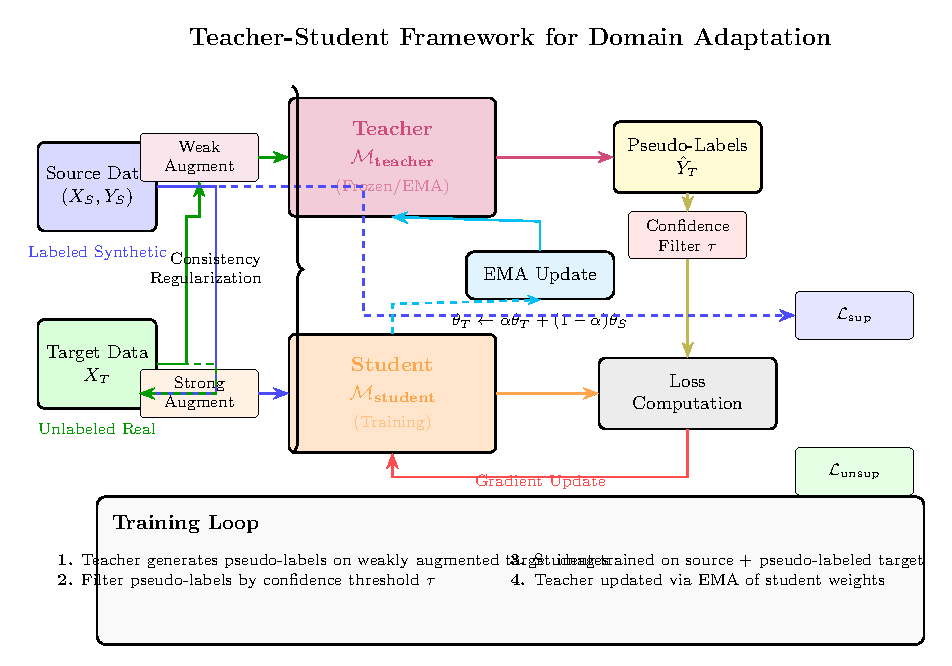
\includegraphics[width=\textwidth]{figures/ch06_fig4_teacher_student.pdf}
\caption{Teacher-student framework for domain adaptation in object detection. The teacher network generates pseudo-labels on weakly augmented target domain images, which are filtered by confidence threshold $\tau$. The student network is trained on both labeled source data (with supervised loss $\mathcal{L}_{\text{sup}}$) and pseudo-labeled target data (with unsupervised loss $\mathcal{L}_{\text{unsup}}$). Strong augmentation is applied to target images before student processing. The teacher weights are updated via exponential moving average (EMA) of student weights, providing stable pseudo-label generation throughout training.}
\label{fig:teacher_student}
\end{figure}

\begin{algorithm}[htbp]
\caption{Teacher-Student Domain Adaptation for Object Detection}
\label{alg:teacher_student}
\begin{algorithmic}[1]
\Require Labeled source data $\mathcal{D}_S = \{(x_S^i, y_S^i)\}$, unlabeled target data $\mathcal{D}_T = \{x_T^j\}$
\Require Pretrained source model $\mathcal{M}_S$, EMA decay rate $\alpha$
\Ensure Target-adapted student model $\mathcal{M}_{\text{student}}$
\State Initialize teacher $\mathcal{M}_{\text{teacher}} \leftarrow \mathcal{M}_S$
\State Initialize student $\mathcal{M}_{\text{student}} \leftarrow \mathcal{M}_S$
\For{epoch $= 1, 2, \ldots, E$}
    \For{each mini-batch $(x_S, y_S) \sim \mathcal{D}_S$, $x_T \sim \mathcal{D}_T$}
        \State \textbf{// Supervised loss on source data}
        \State $\mathcal{L}_{\text{sup}} \leftarrow \mathcal{L}_{\text{det}}(\mathcal{M}_{\text{student}}(x_S), y_S)$
        \State \textbf{// Generate pseudo-labels for target data}
        \State $\hat{y}_T \leftarrow \mathcal{M}_{\text{teacher}}(x_T)$
        \State Filter $\hat{y}_T$ by confidence threshold $\tau$
        \State \textbf{// Apply strong augmentation to target images}
        \State $\tilde{x}_T \leftarrow \text{StrongAugment}(x_T)$
        \State \textbf{// Unsupervised loss with pseudo-labels}
        \State $\mathcal{L}_{\text{unsup}} \leftarrow \mathcal{L}_{\text{det}}(\mathcal{M}_{\text{student}}(\tilde{x}_T), \hat{y}_T)$
        \State \textbf{// Combined loss and student update}
        \State $\mathcal{L} \leftarrow \mathcal{L}_{\text{sup}} + \lambda \mathcal{L}_{\text{unsup}}$
        \State Update $\mathcal{M}_{\text{student}}$ via gradient descent on $\mathcal{L}$
        \State \textbf{// Exponential moving average update for teacher}
        \State $\theta_{\text{teacher}} \leftarrow \alpha \theta_{\text{teacher}} + (1 - \alpha) \theta_{\text{student}}$
    \EndFor
\EndFor
\State \Return $\mathcal{M}_{\text{student}}$
\end{algorithmic}
\end{algorithm}

SF-YOLO represents a state-of-the-art instantiation of teacher-student adaptation for YOLO object detectors. The framework incorporates a Student Stabilization Module that prevents catastrophic forgetting of source domain knowledge during adaptation. Target-specific augmentations applied to student inputs but not teacher inputs encourage the student to develop robustness to target domain variations while maintaining consistency with teacher predictions.

The exponential moving average update for teacher weights provides temporal smoothing that stabilizes pseudo-label quality. The teacher represents an ensemble of student checkpoints weighted toward recent iterations, producing predictions that are more reliable than any single student checkpoint. The EMA decay rate $\alpha$ is typically set between 0.99 and 0.999, with higher values providing greater stability at the cost of slower adaptation to improved student representations.

\section{Measuring and Minimizing Domain Gap}
\label{sec:measuring_gap}

Effective domain adaptation requires methods for assessing the degree of distributional discrepancy and strategies for reducing identified gaps. This section presents approaches for domain gap measurement and gap-aware training methodologies.

\subsection{Domain Discriminator Approaches}

Training a discriminator network to classify features by domain origin provides both a measurement of domain gap and a mechanism for encouraging domain-invariant representations.

As a gap measurement tool, discriminator accuracy indicates the severity of distributional discrepancy. When source and target feature distributions are identical, no classifier can distinguish them better than random chance, yielding approximately fifty percent accuracy. As distributions diverge, discriminator accuracy increases toward perfect classification. The gap between observed accuracy and chance level quantifies the discriminability of domains in feature space.

\begin{figure}[htbp]
\centering
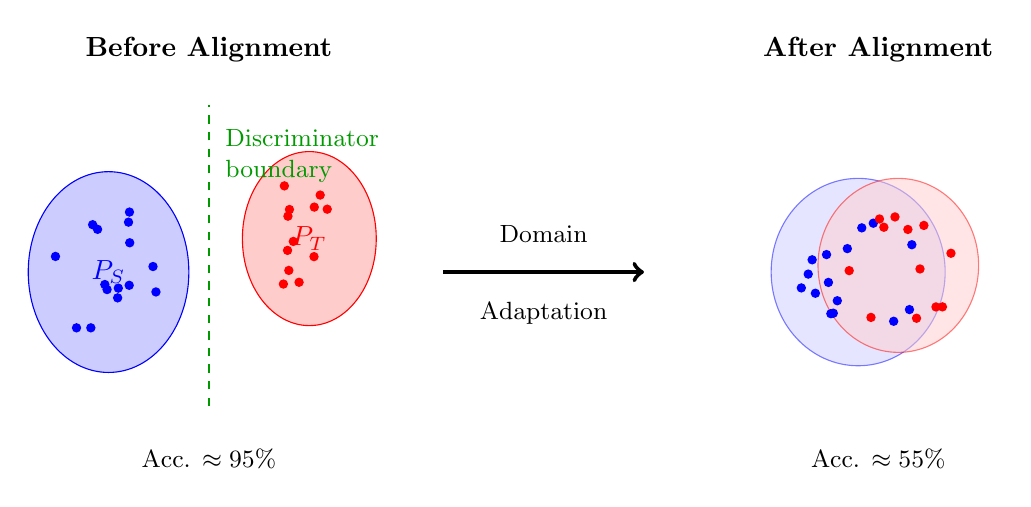
\begin{tikzpicture}[scale=0.85]
    % Feature space before alignment
    \begin{scope}[shift={(-5,0)}]
        \node[above] at (0,3) {\textbf{Before Alignment}};
        % Source cluster (synthetic)
        \draw[fill=blue!20, draw=blue] (-1.5,0) ellipse (1.2 and 1.5);
        \node[blue] at (-1.5,0) {$P_S$};
        % Target cluster (real)
        \draw[fill=red!20, draw=red] (1.5,0.5) ellipse (1.0 and 1.3);
        \node[red] at (1.5,0.5) {$P_T$};
        % Separating hyperplane
        \draw[thick, dashed, green!60!black] (0,-2) -- (0,2.5);
        \node[green!60!black, right] at (0.1,2) {\small Discriminator};
        \node[green!60!black, right] at (0.1,1.5) {\small boundary};
        % Scatter points
        \foreach \i in {1,...,15} {
            \pgfmathsetmacro{\x}{-1.5+0.8*rand}
            \pgfmathsetmacro{\y}{0.9*rand}
            \fill[blue] (\x,\y) circle (2pt);
        }
        \foreach \i in {1,...,12} {
            \pgfmathsetmacro{\x}{1.5+0.6*rand}
            \pgfmathsetmacro{\y}{0.5+0.8*rand}
            \fill[red] (\x,\y) circle (2pt);
        }
        \node[below] at (0,-2.5) {\small Acc. $\approx 95\%$};
    \end{scope}

    % Arrow
    \draw[->, ultra thick] (-1.5,0) -- (1.5,0);
    \node[above] at (0,0.3) {\small Domain};
    \node[below] at (0,-0.3) {\small Adaptation};

    % Feature space after alignment
    \begin{scope}[shift={(5,0)}]
        \node[above] at (0,3) {\textbf{After Alignment}};
        % Overlapping clusters
        \draw[fill=blue!20, draw=blue, opacity=0.5] (-0.3,0) ellipse (1.3 and 1.4);
        \draw[fill=red!20, draw=red, opacity=0.5] (0.3,0.1) ellipse (1.2 and 1.3);
        % Mixed scatter points
        \foreach \i in {1,...,15} {
            \pgfmathsetmacro{\x}{-0.3+0.9*rand}
            \pgfmathsetmacro{\y}{0.9*rand}
            \fill[blue] (\x,\y) circle (2pt);
        }
        \foreach \i in {1,...,12} {
            \pgfmathsetmacro{\x}{0.3+0.8*rand}
            \pgfmathsetmacro{\y}{0.1+0.8*rand}
            \fill[red] (\x,\y) circle (2pt);
        }
        \node[below] at (0,-2.5) {\small Acc. $\approx 55\%$};
    \end{scope}
\end{tikzpicture}
\caption{Domain shift in feature space before and after adaptation. High discriminator accuracy indicates substantial domain gap, while accuracy near chance level indicates well-aligned feature distributions.}
\label{fig:domain_shift}
\end{figure}

Multi-scale discriminators assess domain gap at different levels of feature abstraction. A discriminator operating on early layer features measures low-level appearance discrepancy arising from texture, color, and noise differences. Discriminators on deeper features assess higher-level semantic alignment. Jointly monitoring discriminators across scales provides a comprehensive picture of where domain gap manifests in the learned representation hierarchy.

Class-conditional discriminators separately assess domain gap for each object category. This granular analysis reveals which classes exhibit the largest synthetic-real discrepancy, enabling targeted improvement of synthetic data generation for problematic categories. Classes with high discriminator accuracy require additional variation in synthetic rendering to better match real-world appearance distributions.

\subsection{t-SNE Visualization Analysis}

Visual inspection of feature space structure through t-SNE projection provides intuitive understanding of domain relationships that complements quantitative metrics.

Joint embedding of synthetic and real features enables direct visual comparison of domain distributions. Features are extracted from both domains using the current model, concatenated, and jointly projected to two dimensions via t-SNE. The resulting visualization reveals whether synthetic and real features cluster separately or intermingle. Color-coding by domain origin and object class enables assessment of both domain-level and class-conditional alignment.

Temporal monitoring of t-SNE embeddings throughout training reveals the dynamics of domain adaptation. Initial projections typically show clear separation between synthetic and real clusters. As adaptation progresses, cluster overlap should increase, indicating that the model is learning domain-invariant representations. Failure of clusters to merge despite extended training suggests that the current adaptation approach is insufficient.

Class-specific analysis examines whether certain object categories exhibit greater domain gap than others. Even when overall distributions appear aligned, individual classes may remain separated, indicating that the model has achieved domain invariance for some categories while failing on others. This analysis guides prioritization of synthetic data improvement efforts.

\subsection{Automated Gap Estimation}

Manual inspection of visualizations and discriminator accuracies does not scale to continuous monitoring requirements of automated training systems. Automated gap estimation methods provide scalar metrics suitable for integration into training loops and optimization objectives.

Proxy A-distance provides a computationally efficient approximation to domain discrepancy. Given features from source and target domains, a linear classifier is trained to distinguish them, and the proxy A-distance is computed as $\hat{d}_A = 2(1 - 2\epsilon)$ where $\epsilon$ is the classifier error rate. This metric correlates with theoretical domain adaptation bounds and can be computed with minimal additional computation during training.

Feature distribution moments including mean, variance, and higher-order statistics provide simple gap indicators. The distance between domain-conditional feature means quantified by cosine similarity or Euclidean distance measures first-order distributional discrepancy. Matching variances addresses second-order differences. Maximum Mean Discrepancy provides a principled approach to comparing distributions through all moments via kernel embeddings.

Neural network-based gap estimators can be trained end-to-end to predict transfer performance from feature statistics. Given labeled transfer performance data from previous experiments, a regression network learns to map feature distribution summaries to expected target domain accuracy. Once trained, this predictor provides automated gap estimation for new synthetic data configurations without requiring full transfer evaluation.

\subsection{Gap-Aware Training Strategies}

Domain gap measurements can be integrated into training objectives to explicitly encourage gap minimization alongside task performance optimization.

Multi-objective optimization jointly minimizes task loss and domain discrepancy:
\begin{equation}
\mathcal{L}_{\text{total}} = \mathcal{L}_{\text{task}} + \lambda_{\text{gap}} \mathcal{L}_{\text{gap}}
\end{equation}
where $\mathcal{L}_{\text{task}}$ is the standard detection loss on labeled synthetic data and $\mathcal{L}_{\text{gap}}$ is a differentiable gap metric such as domain discriminator loss or MMD. The weighting parameter $\lambda_{\text{gap}}$ controls the relative importance of task performance versus domain alignment.

Curriculum-based gap reduction schedules the emphasis on gap minimization throughout training. Initial training phases focus primarily on task learning with minimal gap penalty. As task performance saturates, the gap penalty weight is increased to encourage continued domain adaptation. This curriculum prevents premature emphasis on gap reduction before the model has learned task-relevant features to align.

Adaptive weighting schemes adjust gap penalty importance based on current gap magnitude. When domain discrepancy is large, increased gap penalty accelerates alignment. When distributions are already well-aligned, reduced penalty avoids over-regularization that could harm task performance. This adaptive approach automatically balances task and domain objectives throughout training.

Gap-conditional data selection biases synthetic data sampling toward configurations that minimize domain gap. Synthetic images similar to real data under a learned gap metric are preferentially included in training batches. This approach focuses training computation on the most realistic synthetic examples rather than wasting resources on clearly out-of-distribution configurations.

\begin{table}[htbp]
\centering
\caption{Comparison of Domain Adaptation Methods for Object Detection}
\label{tab:da_methods}
\begin{tabular}{p{3cm}p{2.5cm}p{2.5cm}p{2.5cm}p{3cm}}
\toprule
\textbf{Method} & \textbf{Labeled Real Data} & \textbf{Unlabeled Real Data} & \textbf{Computational Cost} & \textbf{Typical Improvement} \\
\midrule
Fourier Domain Adaptation & Not required & Few samples & Very low & 3--8\% mAP \\
\addlinespace
Domain Discriminator & Not required & Recommended & Medium & 5--12\% mAP \\
\addlinespace
CycleGAN Style Transfer & Not required & Required & High & 4--10\% mAP \\
\addlinespace
Self-Training & Not required & Required & Medium & 8--15\% mAP \\
\addlinespace
Teacher-Student & Not required & Required & Medium-High & 10--18\% mAP \\
\addlinespace
Domain Randomization & Not required & Not required & Low & 15--25\% vs. no DR \\
\addlinespace
Fine-tuning on Real & Required & Optional & Low & 20--40\% mAP \\
\bottomrule
\end{tabular}
\end{table}

\section{Summary}

This chapter has provided a comprehensive treatment of domain adaptation and sim-to-real transfer for object detection systems. The domain gap problem arises from systematic differences between synthetic and real image distributions, manifesting in texture, lighting, sensor noise, and contextual composition discrepancies. Formal characterization of domain shift through distributional divergence metrics including FID, KID, and MMD enables quantitative assessment of synthetic data quality and guides optimization of data generation parameters.

Domain randomization provides a principled approach to sim-to-real transfer by training on sufficiently diverse synthetic distributions that encompass real-world conditions. Theoretical analysis establishes transfer bounds relating randomization breadth to expected generalization performance, revealing fundamental tradeoffs between exploration and robustness. Structured domain randomization improves upon uniform approaches by incorporating contextual constraints that focus generated examples on plausible configurations, achieving substantial gains in sample efficiency and transfer performance.

Active and adaptive domain randomization methods learn to optimize randomization parameters based on training feedback. Active Domain Randomization employs discriminative rewards to identify challenging environment configurations. DORAEMON formulates adaptive randomization as constrained entropy maximization, automatically constructing curricula from narrow to broad parameter distributions. These approaches provide principled mechanisms for the reinforcement learning-based optimization of synthetic data generation that motivates this textbook.

Domain adaptation techniques explicitly transform data or representations to reduce distributional discrepancy. Fourier Domain Adaptation transfers low-frequency appearance statistics from real to synthetic images through spectral manipulation. Adversarial feature alignment trains domain-invariant representations through gradient reversal. Teacher-student frameworks enable adaptation using unlabeled target domain data through pseudo-label generation and consistency regularization. The choice among these techniques depends on available data, computational resources, and target performance requirements.

Measuring and minimizing domain gap requires both quantitative metrics and visual analysis tools. Domain discriminator accuracy provides a learned measure of distributional discrepancy. t-SNE visualization enables intuitive assessment of feature space structure. Automated gap estimation methods scale to continuous monitoring requirements of automated training systems. Gap-aware training strategies integrate discrepancy minimization into optimization objectives, ensuring that learned representations achieve both task competence and domain invariance.

The techniques presented in this chapter form the foundation for autonomous optimization of synthetic data generation. By understanding the sources of domain gap, the mechanisms by which randomization enables transfer, and the methods available for measuring and minimizing discrepancy, practitioners can design reinforcement learning systems that automatically discover synthetic data configurations yielding robust real-world performance.
